%Общий объем раздела 15-25 стр. (x2, если разделы объединены)

\section{Описание разработанного программного обеспечения и экспериментальные исследования}

В рамках данной работы были реализованы три модели нейронных сетей для стегоанализа изображений в оттенках серого: GNCNN~\cite{GNCNN}, нейронная сеть с двумя свёрточными слоями~\cite{FrenchCNN} и собственная модель. Впервые были получены свёрточные ИНС для стегоанализа цветных изображений путём модификации вышеперечисленных моделей.

Также была произведена оценка различающей способности данных нейронных сетей.

\subsection{Структура разработанного программного обеспечения}

Модели нейронных сетей реализованы на языке программирования Python и протестированы с использованием интерпретатора Python~3.5.2. Для реализации математического аппарата нейронных сетей использована библиотека Keras~2.2.4~\cite{Keras} и TensorFlow~1.13.1~\cite{TensorFlow}. Для продуцирования графиков --- библиотека livelossplot~0.3.4~\cite{livelossplot}.

\begin{figure}
\centering
\includegraphics[width=1\textwidth]{include/graphics/gncnn_color_architecture}
\caption{Архитектура GNCNN}
\label{fig:GNCNNArchitecture}
\end{figure}

\begin{figure}[!htb]
\centering
\includegraphics[width=1\textwidth]{include/graphics/french_color_architecture}
\caption{Архитектура сети с двумя свёрточными слоями}
\label{fig:FrenchCNNArchitecture}
\end{figure}


\begin{figure}[!htb]
\centering
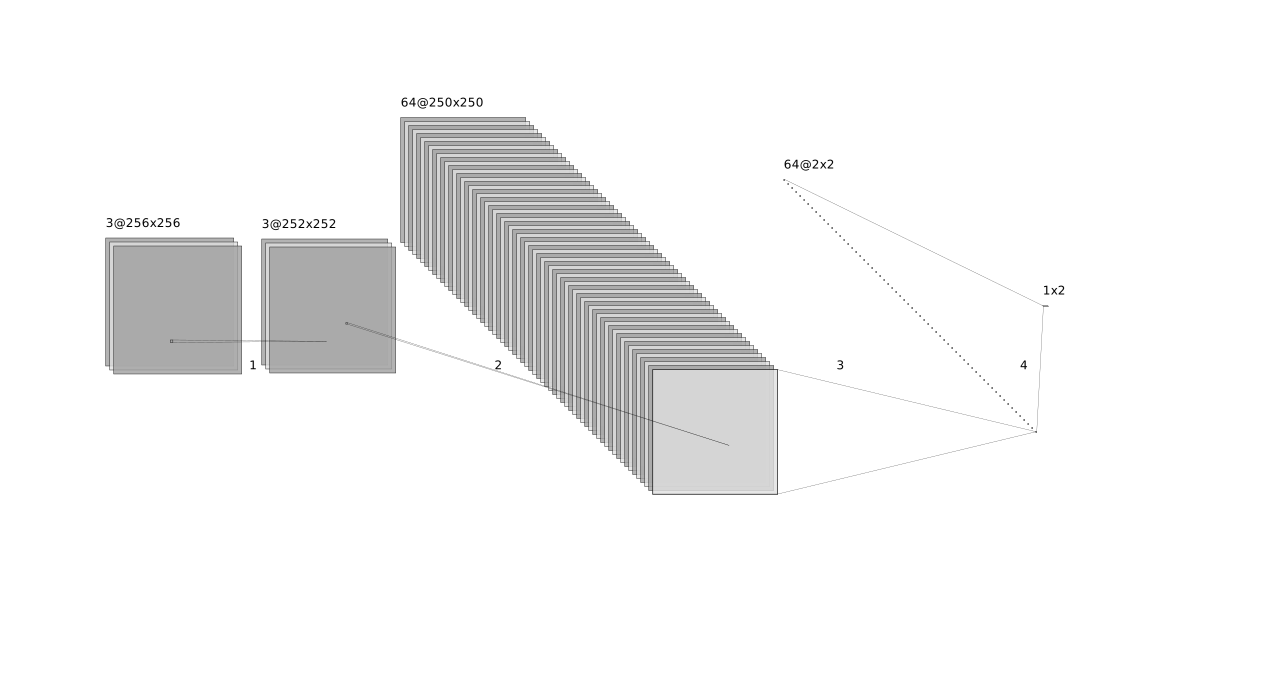
\includegraphics[width=1\textwidth]{include/graphics/mixed_color_architecture}
\caption{Архитектура комбинированной свёрточной сети}
\label{fig:FrenchCNNArchitecture}
\end{figure}
\subsection{Алгоритмы предобработки данных при проведении стегоанализа}

\subsection{Функциональные возможности разработанного программного обеспечения}
\subsection{Интерфейсная часть разработанного программного обеспечения}
\subsection{Перечень алгоритмов стеговстраивания по отношению к которым решалась задача}
\subsection{Описание реализованных алгоритмов стегоанализа}
\subsubsection{Свёрточная нейронная сеть GNCNN}
 В рамках эксперимента использовалось значение $ \sigma = 0,1 $.
 В процессе обучения в качестве функции потерь применялась категориальная кросс-энтропия. Используемый метод обучения – Adam со скоростью обучения 0,001, $ \beta_1 = 0,9 $, $ \beta_2 = 0,999 $. 
\subsection{Результаты сравнительного исследования альтернативных вариантов алгоритмов стегоанализа}

Целью проведения эксперимента было определение способности вышеописанных нейронных сетей различать пустые и заполненные различными способами стегоконтейнеры. Для заполнения использовалось следующее программное обеспечение:

\begin{itemize}
\item программная реализация метода создания цифровых водяных знаков на основе гетероассоциативных сжимающих преобразований (ГСП)~\cite{SirotaHIC};
\item собственная реализация метода относительной замены коэффициентов дискретного косинусного преобразования (ДКП) Коха и Жао~\cite{ZhaoKoch, KochZhao};
\item симулятор стеговстраивания с использованием алгоритма WOW~\cite{WOW}.
\end{itemize}

Для проведения эксперимента использовалась база данных изображений PPG-LIRMM-COLOR~\cite{PPG-LIRMM-COLOR}, состоящая из 10 000 изображений в разрешении 512×512 пикселей. База данных подверглась конвертации в формат изображений в оттенках серого с помощью программы ppmtopgm~\cite{ppmtopgm}. Затем из каждого изображения были вырезаны два фрагмента размером 256×256 пикселей: один из них использовался для обучения нейронной сети сжатия в составе реализации метода создания цифровых водяных знаков на основе ГСП, второй – для осуществления встраивания обученной сетью. В дальнейшем последний фрагмент также использовался для стеговстраивания с применением собственной реализации метода Коха и Жао и симулятора встраивания с использованием алгоритма WOW.

Таким образом, для обучения нейронных сетей были получены три выборки из 10 тыс. пустых и 10 тыс. заполненных одним из перечисленных стегоалгоритмов контейнеров.

Также были сформированы аналогичные выборки из 1 тыс. пустых и 1 тыс. заполненных контейнеров для оценки влияния объёма выборки на точность классификации.

Обучающая подвыборка составила 90~\% полученной выборки, валидационная – 10~\% во всех случаях.

В рамках эксперимента было произведено сравнение реализаций методов стеговстраивания по средней среднеквадратической ошибке и среднему проценту восстановленных посредством стегоизвлечения данных~\ref{table:1}, а также обучение GNCNN и нейронной сети с двумя свёрточными слоями с целью оценки их способности к классификации стегоконтейнеров~\ref{table:2}.

Для каждого стегоалгоритма указан параметр, характеризующий мощность стеговоздействия. Для метода на основе гетероассоциативных сжимающих преобразований им является амплитуда встраивания $ A_m $, для алгоритма Коха и Жао – разность между коэффициентами ДКП $ p $, кодирующая различие между логическими нулём и единицей встраиваемой битовой последовательности, для алгоритма WOW – количество встроенных битов, делённое на количество пикселей в изображении, $ \alpha $.

\begin{table}[h!]
\centering
    \begin{tabular}{| l | l | l |}
    \hline
    Стегоалгоритм & MSE & Процент восстановленных данных \\ \hline
    На основе ГСП ($ A_m = 0,016 $) & 0,1334 & 97,23~\% \\ \hline
    Алгоритм Коха и Жао ($ p = 1 $) & 0,5775 & 99,78~\% \\ \hline
    WOW ($ \alpha = 0,4 $) & 0,0389 & – \\ \hline
%    \hline
    \end{tabular}
\caption{Характеристики реализаций методов встраивания}
\label{table:1}
\end{table}

\begin{table}[h!]
\centering
    \begin{tabular}{| l | l | l |}
    \hline
    Стегоалгоритм & MSE & Процент восстановленных данных \\ \hline
    На основе ГСП ($ A_m = 0,016 $) & 0.0475 & 98,79~\% \\ \hline
    Алгоритм Коха и Жао ($ p = 1 $) & 0.1995 & 99,76~\% \\ \hline
    WOW ($ \alpha = 0,4 $) & 0.0129 & – \\ \hline
%    \hline
    \end{tabular}
\caption{Характеристики реализаций методов встраивания}
\label{table:1Color}
\end{table}

Процент успешно извлечённых после стеговстраивания данных для алгоритма WOW не указан ввиду использования симулятора, не производящего сокрытия информации, а лишь изменяющего пиксели соответственно алгоритму встраивания.
\begin{landscape}

\begin{table}[h!]
\centering
    \begin{tabular}{| l | p{2cm} | p{2cm} | p{2cm} | p{2cm} | p{2cm} | p{2cm} |}
    \hline
    Стегоалгоритм & GNCNN (2 K) & GNCNN (20 K) & 2\=/хслойная НС (2 тыс.) & 2\=/хслойная НС (20 тыс.) & Моя НС (2 тыс.) & Моя НС (20 тыс.) \\ \hline
    На основе ГСП ($ A_m = 0,016 $) & 94,1~\% & 96,8~\% & 48~\% & 51,7~\% & 96~\% & 95,1~\% \\ \hline
    Алгоритм Коха и Жао ($ p = 1 $) & 50,7~\% & 93,1~\% & 100~\% & 99,8~\% & 100~\% & 99~\% \\ \hline
    WOW ($ \alpha = 0,4 $) & 50~\% & 49,6~\% & 85,5~\% & 96,3~\% & 92,5~\% & 95~\% \\ \hline
    \end{tabular}
\caption{Точность классификации стегоконтейнеров валидационной подвыборки}
\label{table:2}
\end{table}

\begin{table}[h!]
\centering
    \begin{tabular}{| l | p{2cm} | p{2cm} | p{2cm} | p{2cm} | p{2cm} | p{2cm} |}
    \hline
    Стегоалгоритм & GNCNN (2 K) & GNCNN (20 K) & 2\=/хслойная НС (2 тыс.) & 2\=/хслойная НС (20 тыс.) & Моя НС (2 тыс.) & Моя НС (20 тыс.) \\ \hline
    На основе ГСП ($ A_m = 0,016 $) & 53,7~\% & 99,5~\% & 50~\% & 50~\% & 82,5~\% & 100~\% \\ \hline
    Алгоритм Коха и Жао ($ p = 1 $) & 49,3~\% & 49,1~\% & 99,5~\% & 100~\% & 98~\% & 98,1~\% \\ \hline
    WOW ($ \alpha = 0,4 $) & 50~\% & 49,4~\% & 54,5~\% & 96,7~\% & 90~\% & 91,1~\% \\ \hline
    \end{tabular}
\caption{Точность классификации стегоконтейнеров валидационной подвыборки}
\label{table:2}
\end{table}
\end{landscape}

Из~\ref{table:2} видно, что обе нейронные сети имеют практически одинаковую способность к различению пустых стегоконтейнеров и стегоконтейнеров, заполненных с помощью реализации метода Коха и Жао, на выборке из 20 тыс. изображений.

Однако успешно детектировать заполненные с помощью реализации метода на основе ГСП стегоконтейнеры оказалась способна только GNCNN, в то время как детектирование заполненных с применением симулятора встраивания WOW контейнеров успешно производит только нейронная сеть с двумя свёрточными слоями.

\begin{figure}[p]
    \centering
%    \vspace{30mm}
    \begin{subfigure}[b]{0.485\textwidth}
        \includegraphics[width=\textwidth]{include/graphics/experimental_plots/grayscale/gncnn_hic}
                    \caption{Изменение электрического поля во времени (без PML)}
    \end{subfigure}
    ~
    \begin{subfigure}[b]{0.485\textwidth}
        \includegraphics[width=\textwidth]{include/graphics/experimental_plots/grayscale/mixed_hic}
                    \caption{Изменение электрического поля во времени (без PML)}
    \end{subfigure}
\bigskip
    \begin{subfigure}[b]{0.485\textwidth}
        \includegraphics[width=\textwidth]{include/graphics/experimental_plots/grayscale/gncnn_koch}
                    \caption{Изменение электрического поля во времени (без PML)}
    \end{subfigure}
    ~
    \begin{subfigure}[b]{0.485\textwidth}
        \includegraphics[width=\textwidth]{include/graphics/experimental_plots/grayscale/mixed_koch}
                    \caption{Изменение электрического поля во времени (без PML)}
    \end{subfigure}
    
\bigskip
    \begin{subfigure}[b]{0.485\textwidth}
        \includegraphics[width=\textwidth]{include/graphics/experimental_plots/grayscale/french_wow}
                    \caption{Изменение электрического поля во времени (без PML)}
    \end{subfigure}
    ~
    \begin{subfigure}[b]{0.485\textwidth}
        \includegraphics[width=\textwidth]{include/graphics/experimental_plots/grayscale/mixed_wow}
            \caption{Изменение электрического поля во времени (без PML)}
    \end{subfigure}

    \caption{Изменение электрического поля во времени (без PML)}\label{fig:EzPmlOff}
\end{figure}

\begin{figure}[p]
    \centering
%    \vspace{30mm}
    \begin{subfigure}[b]{0.485\textwidth}
        \includegraphics[width=\textwidth]{include/graphics/experimental_plots/color/gncnn_hic}
    \end{subfigure}
    ~
    \begin{subfigure}[b]{0.485\textwidth}
        \includegraphics[width=\textwidth]{include/graphics/experimental_plots/color/mixed_hic}
    \end{subfigure}
\bigskip
    \begin{subfigure}[b]{0.485\textwidth}
        \includegraphics[width=\textwidth]{include/graphics/experimental_plots/color/french_koch}
    \end{subfigure}
    ~
    \begin{subfigure}[b]{0.485\textwidth}
        \includegraphics[width=\textwidth]{include/graphics/experimental_plots/color/mixed_koch}
    \end{subfigure}
    
\bigskip
    \begin{subfigure}[b]{0.485\textwidth}
        \includegraphics[width=\textwidth]{include/graphics/experimental_plots/color/french_wow}
    \end{subfigure}
    ~
    \begin{subfigure}[b]{0.485\textwidth}
        \includegraphics[width=\textwidth]{include/graphics/experimental_plots/color/mixed_wow}
    \end{subfigure}

    \caption{Изменение электрического поля во времени (без PML)}\label{fig:EzPmlOff}
\end{figure}

\clearpage
